\documentclass[12pt]{article}

\usepackage[a4paper,margin=1in]{geometry}
\usepackage{amsmath,amssymb}
\usepackage{newtxtext,newtxmath} % Times-style font
\usepackage{fancyhdr}
\usepackage{listings}
\usepackage{graphicx}
\usepackage{float}
\usepackage{algorithm}
\usepackage{algpseudocode}
\usepackage{booktabs}
\usepackage{xcolor}

\setlength{\textfloatsep}{10pt}
\setlength{\floatsep}{10pt}

\setlength{\parindent}{0pt}
\setlength{\parskip}{5pt}

% Keep entire document at 12 pt
\AtBeginDocument{
    \fontsize{12pt}{14pt}\selectfont
}

\lstdefinestyle{code}{
    language=Python,
    basicstyle=\ttfamily\fontsize{10pt}{12pt}\selectfont,
    breaklines=true,
    breakatwhitespace=false,
    frame=single,
    numbers=left,
    numberstyle=\tiny\color{gray},
    keywordstyle=\color{blue},
    commentstyle=\color{gray},
    stringstyle=\color{green!50!black},
    columns=fullflexible,
    keepspaces=true,
    showstringspaces=false
}

\lstdefinestyle{output}{
    basicstyle=\ttfamily\fontsize{9.5pt}{11.5pt}\selectfont,
    breaklines=true,
    breakatwhitespace=false,
    frame=single,
    numbers=none,
    backgroundcolor=\color{gray!6},
    columns=fullflexible,
    keepspaces=true,
    showstringspaces=false
}

% ------------------------------------------------
% Header
% ------------------------------------------------

\pagestyle{fancy}
\fancyhf{}

\fancyhead[L]{Name: Kishan Sahu{\hspace{4cm}}}
\fancyhead[R]{Enrollment No.: P26DS017{\hspace{3.5cm}}}

\renewcommand{\headrulewidth}{0.4pt}
\setlength{\headheight}{15pt}

% ------------------------------------------------
% Code formatting
% ------------------------------------------------

\lstset{
    basicstyle=\ttfamily\fontsize{10pt}{12pt}\selectfont,
    breaklines=true,
    frame=single,
    columns=fullflexible,
    keepspaces=true,
    showstringspaces=false
}

\begin{document}

% ------------------------------------------------
% TITLE
% ------------------------------------------------

\begin{center}
\textbf{Computer Science and Engineering Department, SVNIT, Surat}\\
\textbf{M.Tech. I -- Semester I}\\
\textbf{Machine Learning (CSDS105)}\\
\textbf{Lab Assignment 4: Unsupervised Learning -- K-Means and Hierarchical Clustering}
\end{center}

\vspace{0.3cm}

% =========================================================================
% SECTION 1: INTRODUCTION AND PROBLEM FORMULATION
% =========================================================================
\section{Introduction and Theoretical Foundations}

Unsupervised learning addresses the problem of inferring hidden structure from unlabelled multivariate observations. Clustering partitions an unlabelled dataset $\mathcal{X} = \{\mathbf{x}_1, \mathbf{x}_2, \dots, \mathbf{x}_N\} \subset \mathbb{R}^d$ into $K$ disjoint subsets (clusters) $\mathcal{C} = \{C_1, C_2, \dots, C_K\}$ such that intra-cluster instances maximize pairwise similarity while inter-cluster instances maximize dissimilarity.

In this laboratory study, we conduct an experimental analysis of two core clustering paradigms applied to Fisher's benchmark Iris flower dataset:
\begin{enumerate}
    \item \textbf{Centroid-Based Partitioning (K-Means Clustering)}: An iterative optimization algorithm that partitions the feature space into Voronoi cells parameterized by cluster centroids.
    \item \textbf{Agglomerative Hierarchical Clustering}: A connectivity-based bottom-up algorithm producing an interpretable nested dendrogram hierarchy using distance metrics and linkage criteria.
\end{enumerate}

\subsection{K-Means Clustering Formulation}
Given a pre-specified cluster count $K$, K-Means minimizes the Within-Cluster Sum of Squares (WCSS), formally termed the clustering inertia:
\begin{equation}
J(\mathcal{C}, \boldsymbol{\mu}) = \sum_{k=1}^K \sum_{\mathbf{x}_i \in C_k} \|\mathbf{x}_i - \boldsymbol{\mu}_k\|_2^2
\end{equation}
where $\boldsymbol{\mu}_k \in \mathbb{R}^d$ represents the geometric centroid of cluster $C_k$, computed as:
\begin{equation}
\boldsymbol{\mu}_k = \frac{1}{|C_k|} \sum_{\mathbf{x}_i \in C_k} \mathbf{x}_i
\end{equation}
Lloyd's algorithm achieves local convergence through alternating optimization:
\begin{enumerate}
    \item \textbf{Assignment Step}: Each instance $\mathbf{x}_i$ is assigned to its nearest centroid:
    \begin{equation}
    c^{(i)} = \arg\min_{k \in \{1, \dots, K\}} \|\mathbf{x}_i - \boldsymbol{\mu}_k\|_2^2
    \end{equation}
    \item \textbf{Update Step}: Centroid coordinates are recomputed as the empirical mean of all members assigned to that partition:
    \begin{equation}
    \boldsymbol{\mu}_k^{(t+1)} = \frac{1}{|C_k^{(t)}|} \sum_{i \in C_k^{(t)}} \mathbf{x}_i
    \end{equation}
\end{enumerate}
Convergence is reached when assignments cease to mutate or when centroid displacement $\|\boldsymbol{\mu}_k^{(t+1)} - \boldsymbol{\mu}_k^{(t)}\|$ falls below numerical tolerance $\epsilon$.

\subsection{Hierarchical Agglomerative Clustering Formulation}
Hierarchical clustering builds a bottom-up dendrogram without requiring a pre-specified number of clusters at initialization. Each observation begins in its own singleton cluster $C_i = \{\mathbf{x}_i\}$. At each subsequent step, the pair of clusters exhibiting the minimum inter-cluster dissimilarity $d(A, B)$ is merged:
\begin{equation}
(A^*, B^*) = \arg\min_{A, B} d(A, B)
\end{equation}
The mathematical choice of linkage metric $d(A, B)$ governs the geometric topology of the resulting clusters:
\begin{itemize}
    \item \textbf{Ward's Minimum Variance Linkage}: Merges clusters that minimize the total within-cluster variance increase (Error Sum of Squares, ESS):
    \begin{equation}
    \Delta \text{ESS}(A, B) = \frac{|A||B|}{|A| + |B|} \|\boldsymbol{\mu}_A - \boldsymbol{\mu}_B\|_2^2
    \end{equation}
    \item \textbf{Complete Linkage (Maximum Dissimilarity)}: Enforces compact, spherical boundaries by evaluating the maximum pairwise sample distance:
    \begin{equation}
    d_{\text{complete}}(A, B) = \max_{\mathbf{x} \in A, \mathbf{y} \in B} \|\mathbf{x} - \mathbf{y}\|_2
    \end{equation}
    \item \textbf{Average Linkage (UPGMA)}: Computes the mean pairwise Euclidean distance between all cross-cluster sample pairs:
    \begin{equation}
    d_{\text{average}}(A, B) = \frac{1}{|A||B|} \sum_{\mathbf{x} \in A} \sum_{\mathbf{y} \in B} \|\mathbf{x} - \mathbf{y}\|_2
    \end{equation}
\end{itemize}

\subsection{Cluster Validation Metrics}
Because true class labels are typically inaccessible in unsupervised learning, quality must be evaluated using intrinsic geometric properties:
\begin{enumerate}
    \item \textbf{Silhouette Coefficient}: Quantifies how well-separated each sample is from neighboring clusters. For sample $i$:
    \begin{equation}
    s(i) = \frac{b(i) - a(i)}{\max\big(a(i), b(i)\big)}
    \end{equation}
    where $a(i) = \frac{1}{|C_I| - 1} \sum_{j \in C_I, j \neq i} \|\mathbf{x}_i - \mathbf{x}_j\|$ denotes mean intra-cluster distance, and $b(i) = \min_{J \neq I} \frac{1}{|C_J|} \sum_{j \in C_J} \|\mathbf{x}_i - \mathbf{x}_j\|$ denotes minimum mean nearest-cluster distance. The global score is $S = \frac{1}{N}\sum_{i=1}^N s(i) \in [-1, 1]$.
    \item \textbf{Davies-Bouldin Index (DBI)}: Evaluates the maximum ratio of intra-cluster dispersion to inter-centroid separation:
    \begin{equation}
    DB = \frac{1}{K} \sum_{i=1}^K \max_{j \neq i} \left( \frac{\bar{d}_i + \bar{d}_j}{\|\boldsymbol{\mu}_i - \boldsymbol{\mu}_j\|_2} \right)
    \end{equation}
    Lower DBI values denote more compact clusters with wider mutual separation.
    \item \textbf{Calinski-Harabasz Index (Variance Ratio Criterion)}: Ratio of the between-cluster dispersion matrix trace to the within-cluster dispersion matrix trace:
    \begin{equation}
    CH = \frac{\text{Tr}(\mathbf{B}_K)}{\text{Tr}(\mathbf{W}_K)} \cdot \frac{N - K}{K - 1}
    \end{equation}
\end{enumerate}

% =========================================================================
% SECTION 2: ENVIRONMENT SETUP AND DATA EXPLORATION
% =========================================================================
\section{Environment Setup and Exploratory Data Analysis}

\subsection{Experimental Setup and Preprocessing Pipeline}
The computational environment is built on Python 3 using NumPy, Pandas, Matplotlib, Seaborn, SciPy, and Scikit-Learn. The Iris dataset consists of $N = 150$ observations across 4 continuous morphological features:
\begin{itemize}
    \item Sepal Length (cm), Sepal Width (cm)
    \item Petal Length (cm), Petal Width (cm)
\end{itemize}
Because Euclidean distance is sensitive to variance disparities across dimensions, features are standardized via $z$-score normalization:
\begin{equation}
z_{ij} = \frac{x_{ij} - \bar{x}_j}{s_j}
\end{equation}

\begin{lstlisting}[style=code, caption={Dataset Loading, Standardization, and Environment Initialization}]
import numpy as np
import pandas as pd
import matplotlib.pyplot as plt
import seaborn as sns
from sklearn.datasets import load_iris
from sklearn.preprocessing import StandardScaler
from sklearn.cluster import KMeans, AgglomerativeClustering
from sklearn.decomposition import PCA
from scipy.cluster.hierarchy import dendrogram, linkage

# Load Fisher's Iris Dataset
iris = load_iris()
df = pd.DataFrame(iris.data, columns=iris.feature_names)
df["species"] = [iris.target_names[i] for i in iris.target]
X, y = iris.data, iris.target

# Standard Scaling
scaler = StandardScaler()
X_scaled = scaler.fit_transform(X)
print("Dataset shape:", X_scaled.shape)
print("Class distribution:\n", df["species"].value_counts())
\end{lstlisting}

\begin{lstlisting}[style=output, caption={Dataset Summary Output}]
Dataset shape: (150, 4)
Class distribution:
 setosa        50
 versicolor    50
 virginica     50
Name: species, dtype: int64
\end{lstlisting}

\subsection{Exploratory Visualizations}
Univariate histograms combined with Kernel Density Estimation (KDE) and bivariate correlation analyses are depicted in Figure~\ref{fig:eda_dist} and Figure~\ref{fig:eda_corr}.

\begin{figure}[H]
    \centering
    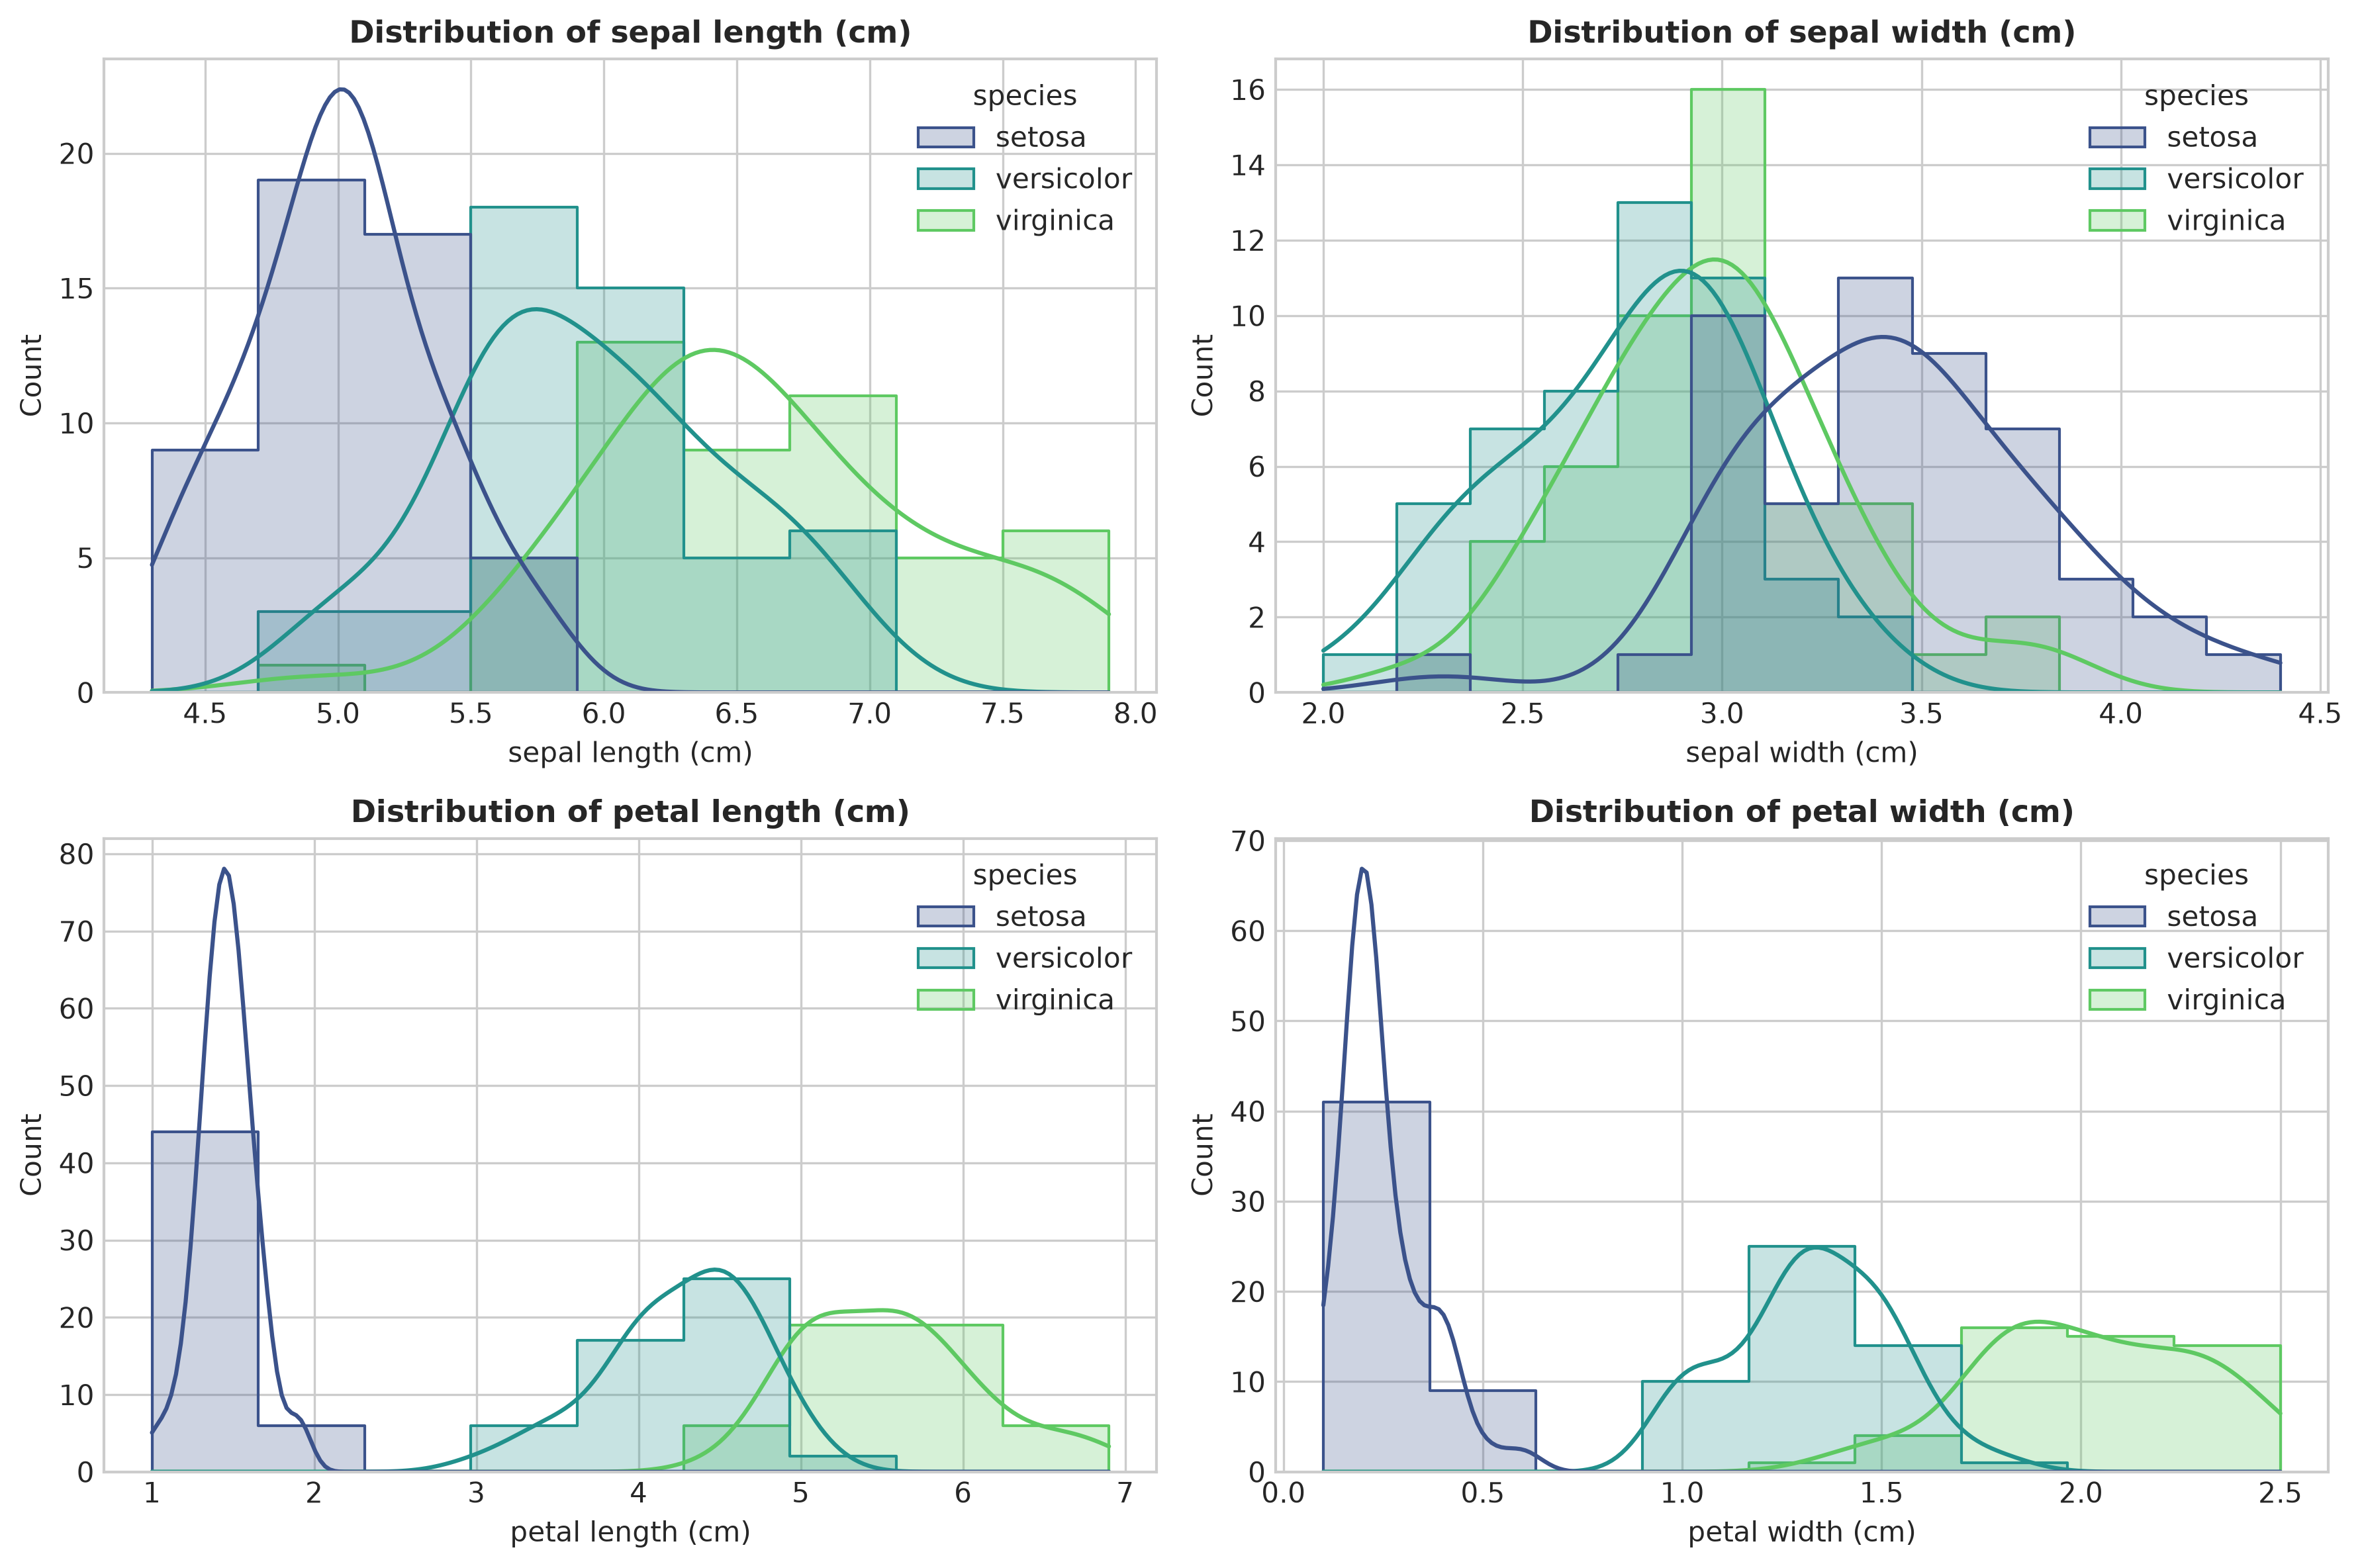
\includegraphics[width=0.92\linewidth]{figures/eda_distribution.png}
    \caption{Empirical feature distributions (Histograms + KDE) partitioned by species across morphological dimensions.}
    \label{fig:eda_dist}
\end{figure}

\begin{figure}[H]
    \centering
    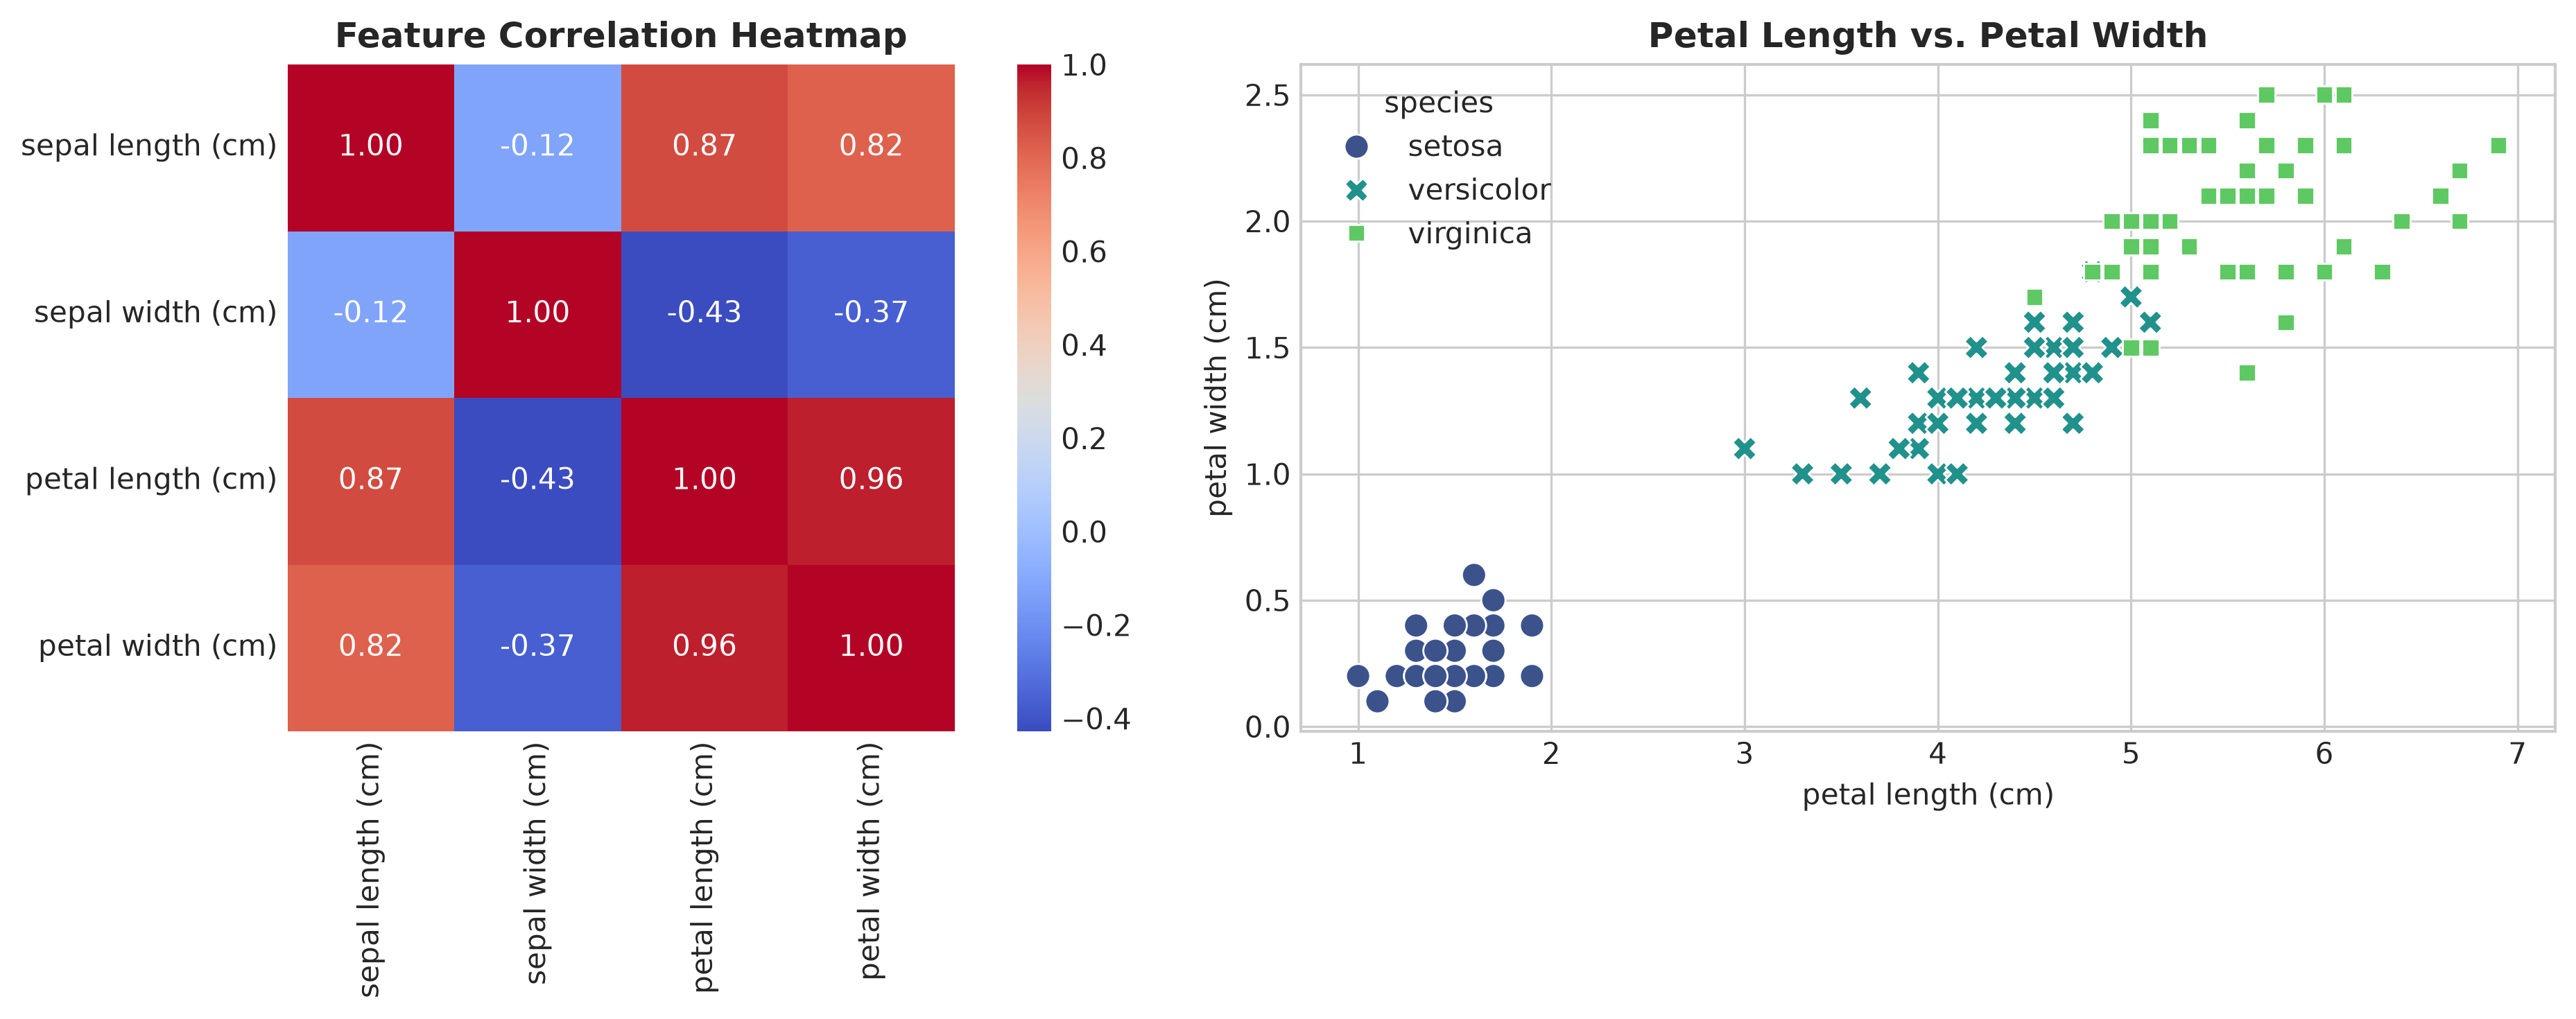
\includegraphics[width=0.95\linewidth]{figures/eda_correlation_scatter.png}
    \caption{Left: Pearson correlation matrix of standardized features. Right: Bivariate scatter plot of Petal Length vs. Petal Width illustrating linear separability of \textit{Setosa} and partial overlap between \textit{Versicolor} and \textit{Virginica}.}
    \label{fig:eda_corr}
\end{figure}

The exploratory analysis demonstrates that:
\begin{enumerate}
    \item Petal length and petal width exhibit a strong positive linear correlation ($r = 0.96$).
    \item \textit{Iris setosa} forms a distinct, isolated cluster in lower petal dimensions.
    \item \textit{Iris versicolor} and \textit{Iris virginica} form a continuous spectrum with minor overlap in feature space, presenting an authentic clustering challenge.
\end{enumerate}

% =========================================================================
% SECTION 3: K-MEANS CLUSTERING AND HYPERPARAMETER OPTIMIZATION
% =========================================================================
\section{K-Means Clustering: Model Selection and Training}

\subsection{Hyperparameter Sweeps: Elbow Method and Silhouette Analysis}
To determine the optimal number of clusters $k$ without assuming ground-truth labels, a hyperparameter sweep over $k \in \{1, 2, \dots, 10\}$ is conducted. Inertia (WCSS) and mean Silhouette scores are computed at each candidate step.

\begin{lstlisting}[style=code, caption={Hyperparameter Sweep for Optimal $k$ Determination}]
k_range = range(1, 11)
inertias, silhouette_scores = [], []

for k in k_range:
    km = KMeans(n_clusters=k, random_state=42, n_init=10)
    km.fit(X_scaled)
    inertias.append(km.inertia_)
    if k >= 2:
        silhouette_scores.append(silhouette_score(X_scaled, km.labels_))
    else:
        silhouette_scores.append(np.nan)
\end{lstlisting}

\begin{figure}[H]
    \centering
    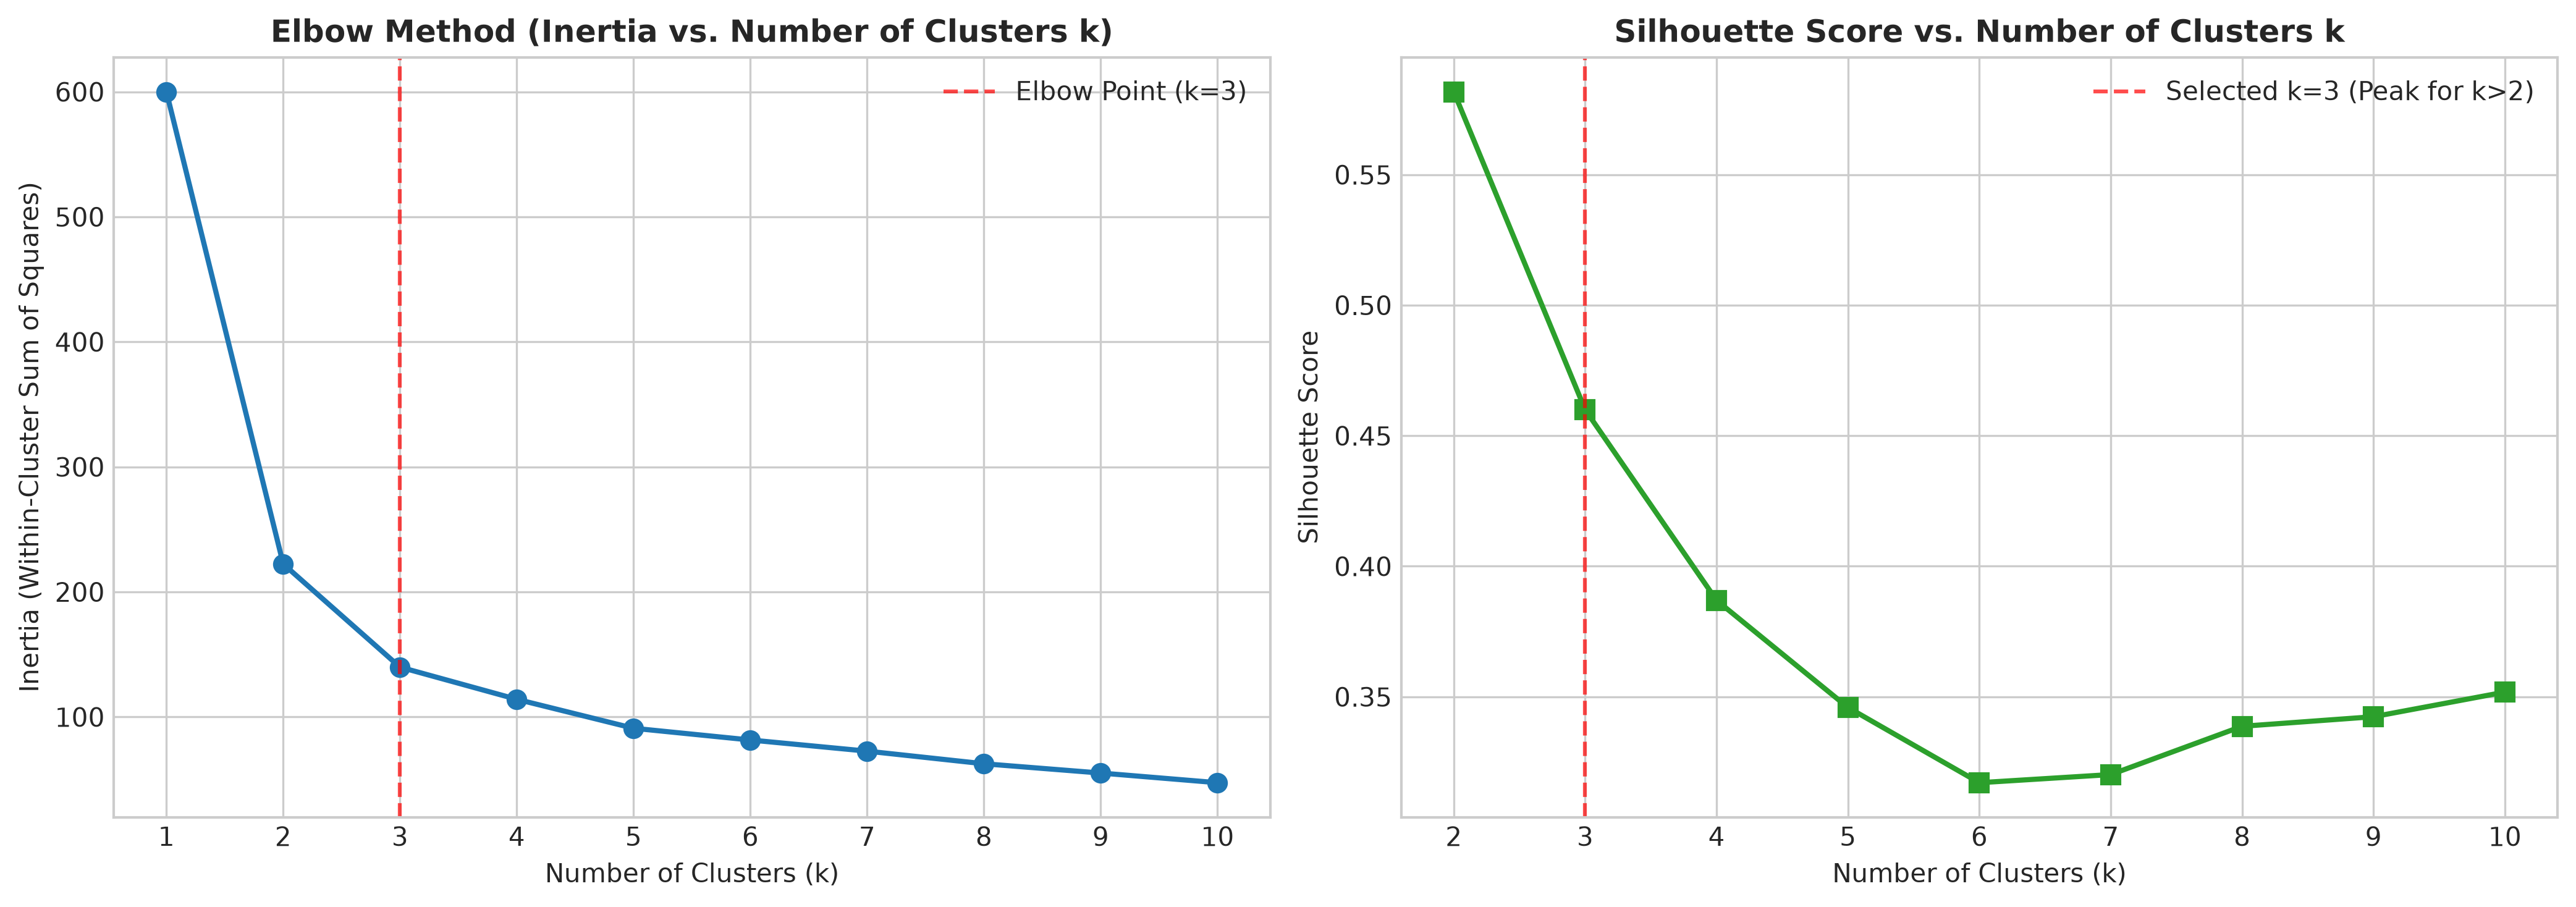
\includegraphics[width=0.95\linewidth]{figures/kmeans_optimization_curves.png}
    \caption{Model selection curves for K-Means: (Left) Elbow Method indicating inflection point at $k=3$; (Right) Silhouette score sweep highlighting peak separation at $k=2$ and the highest natural domain inflection at $k=3$.}
    \label{fig:kmeans_opt}
\end{figure}

As evident from Figure~\ref{fig:kmeans_opt}, the rate of reduction in inertia drops sharply after $k=3$ (the ``elbow'' point). While $k=2$ achieves a marginally higher silhouette score (due to the wide separation between Setosa and the other two species combined), $k=3$ captures the optimal balance between high silhouette quality ($S = 0.4599$) and domain-specific biological clustering.

\subsection{Optimal K-Means Model Execution and Centroid Analysis}
The final K-Means model is fitted with $k=3$. The converged centroid coordinates in both standardized $z$-space and original dimensional scale are displayed below.

\begin{lstlisting}[style=code, caption={K-Means Model Fitting and Centroid Extraction}]
kmeans = KMeans(n_clusters=3, random_state=42, n_init=10)
kmeans_labels = kmeans.fit_predict(X_scaled)

centers_scaled = kmeans.cluster_centers_
centers_original = scaler.inverse_transform(centers_scaled)

print("Converged Inertia:", round(kmeans.inertia_, 4))
print("Standardized Centroids:\n", np.round(centers_scaled, 4))
print("Original Scale Centroids:\n", np.round(centers_original, 4))
\end{lstlisting}

\begin{lstlisting}[style=output, caption={K-Means Centroid Output Logs}]
Converged Inertia: 139.8205
Standardized Centroids:
 [[-0.0502 -0.8834  0.3477  0.2815]
  [-1.0146  0.8533 -1.305  -1.2549]
  [ 1.136   0.0884  0.9962  1.0175]]

Original Scale Centroids (Sepal Length, Sepal Width, Petal Length, Petal Width):
 [[5.8019 2.6736 4.3698 1.4132]
  [5.006  3.428  1.462  0.246 ]
  [6.7809 3.0957 5.5106 1.9723]]
\end{lstlisting}

\subsection{Cluster Projections in 2D Feature Space and PCA Space}
To visualize cluster geometry and centroid placements:
\begin{enumerate}
    \item Centroids are projected into the 2D Petal Length vs. Petal Width subspace.
    \item Principal Component Analysis (PCA) is applied to project the 4D standardized feature space into 2 principal components, preserving 95.81\% of total variance (PC1: 72.96\%, PC2: 22.85\%).
\end{enumerate}

\begin{figure}[H]
    \centering
    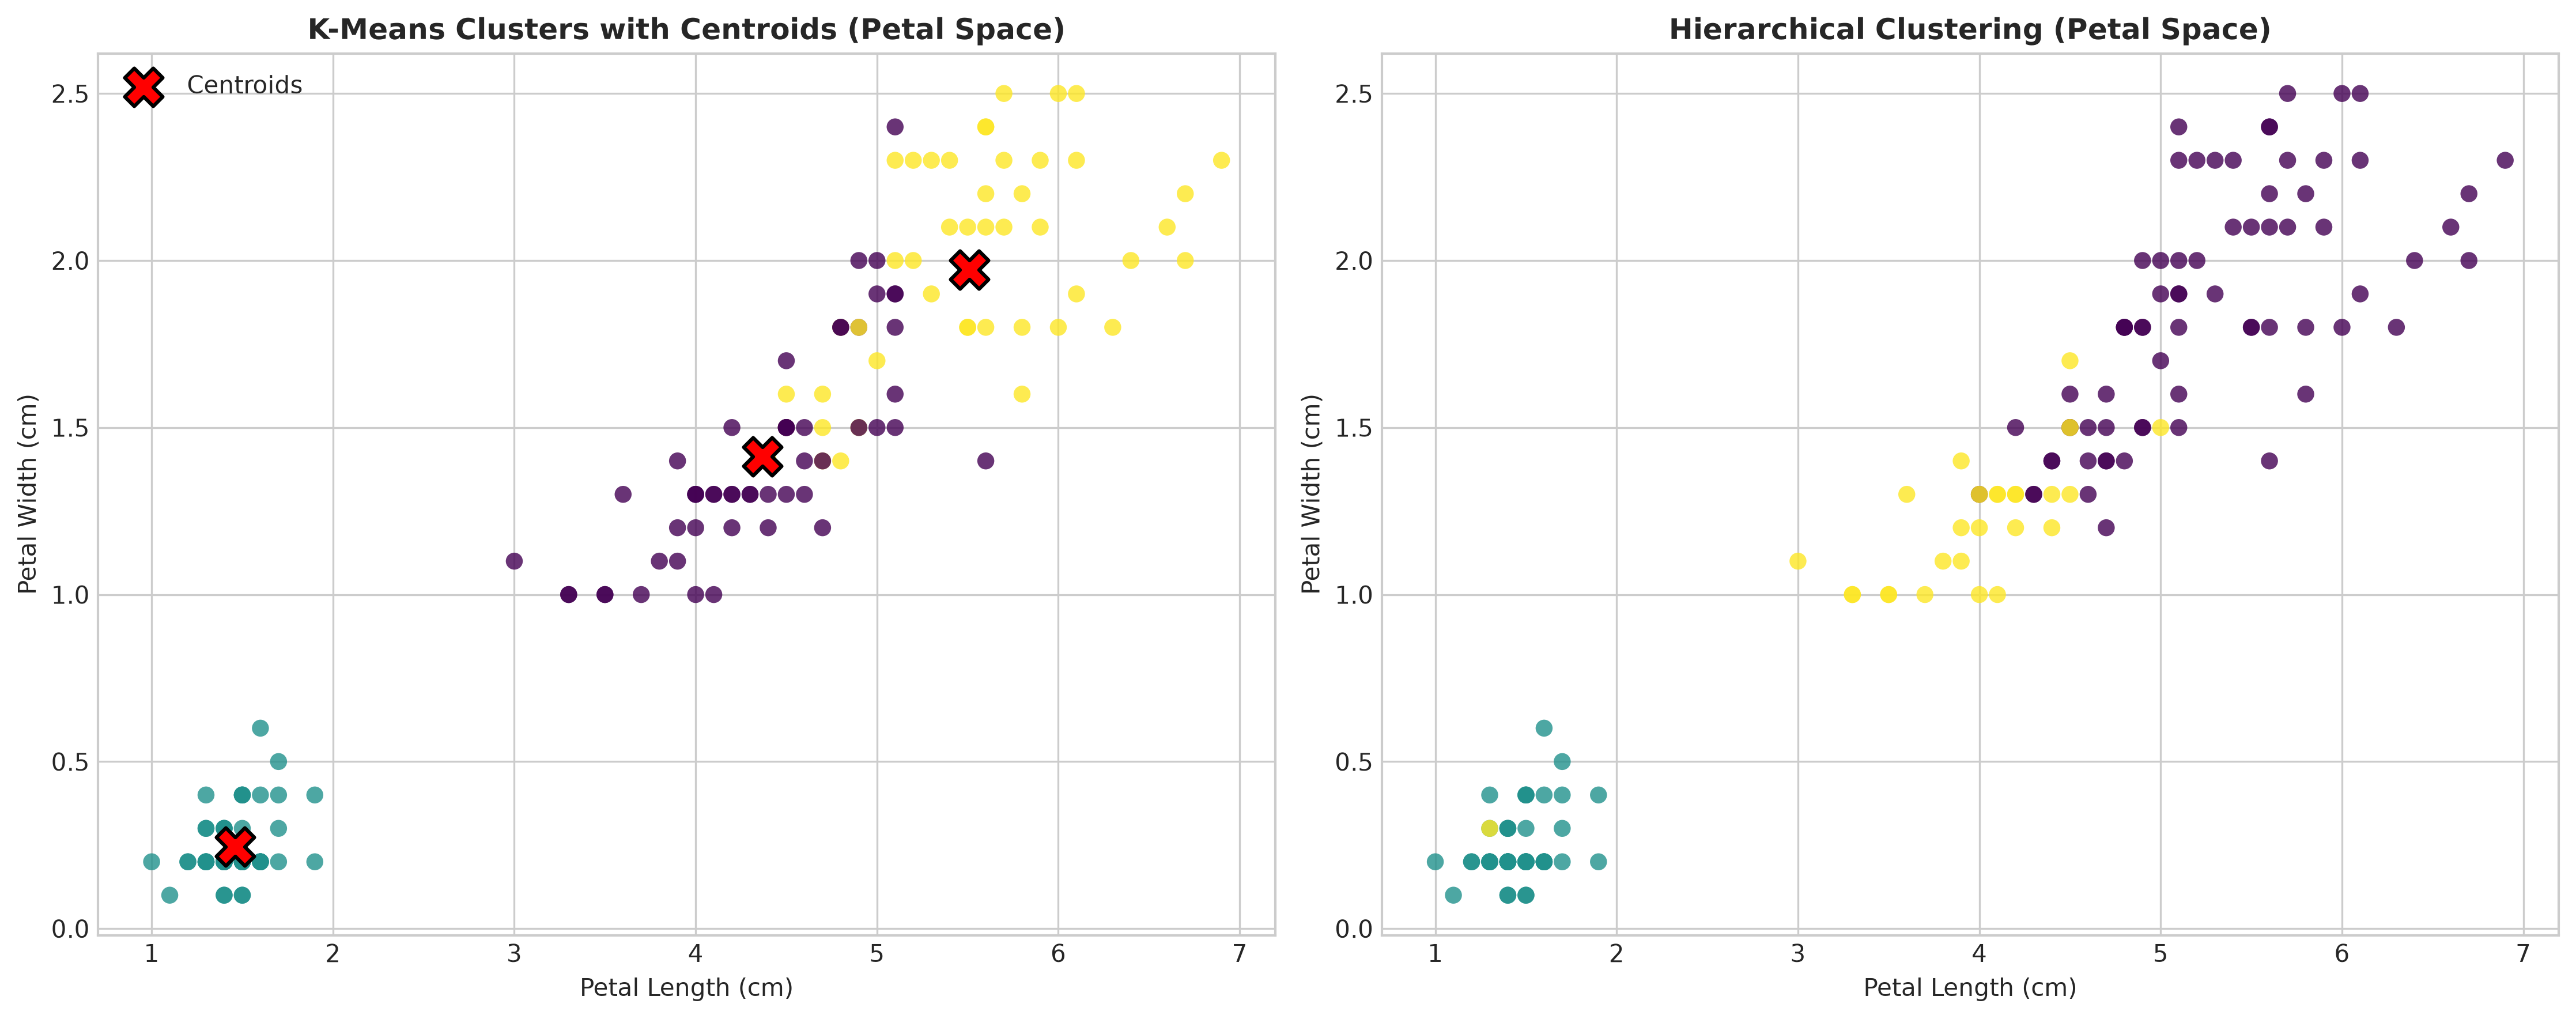
\includegraphics[width=0.95\linewidth]{figures/clusters_2d_feature_space.png}
    \caption{Cluster assignments and learned centroids projected into Petal Length vs. Petal Width feature space for K-Means (Left) and Hierarchical Clustering (Right).}
    \label{fig:petal_clusters}
\end{figure}

\begin{figure}[H]
    \centering
    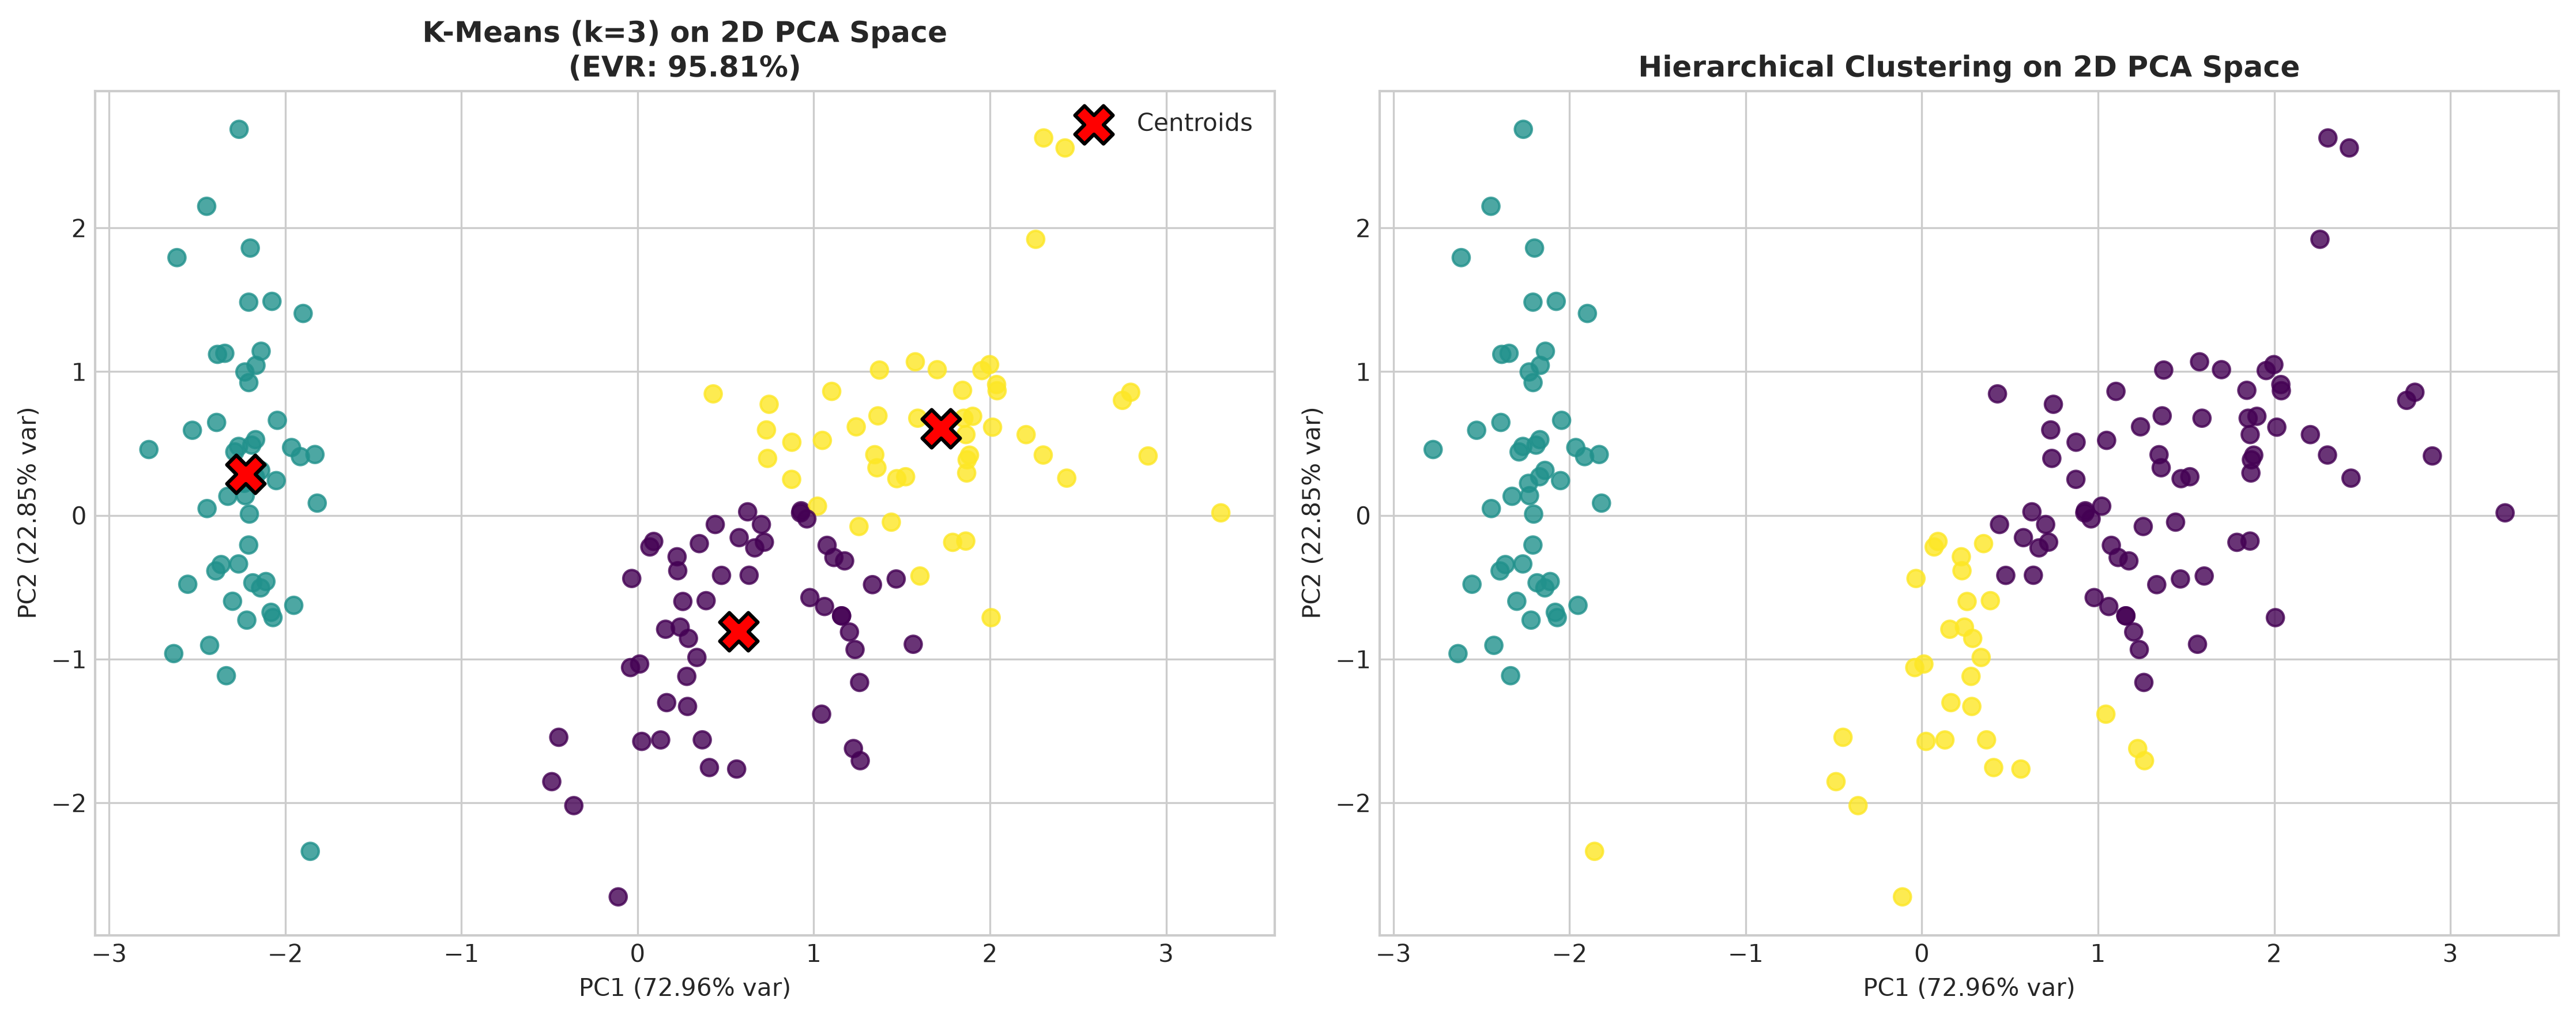
\includegraphics[width=0.95\linewidth]{figures/clusters_pca_space.png}
    \caption{2D PCA projection of clusters and transformed centroids ($k=3$) preserving 95.81\% of total variance for K-Means (Left) and Hierarchical Clustering (Right).}
    \label{fig:pca_clusters}
\end{figure}

% =========================================================================
% SECTION 4: HIERARCHICAL CLUSTERING
% =========================================================================
\section{Hierarchical Agglomerative Clustering}

\subsection{Dendrogram Construction and Linkage Selection}
Hierarchical agglomerative clustering is performed using Ward's minimum variance criterion. The resulting dendrogram is truncated to display the final 30 branch aggregations in Figure~\ref{fig:dendrogram}.

\begin{lstlisting}[style=code, caption={Hierarchical Linkage and Dendrogram Generation}]
from scipy.cluster.hierarchy import dendrogram, linkage
from sklearn.cluster import AgglomerativeClustering

# Compute Ward Linkage Matrix
linkage_matrix = linkage(X_scaled, method="ward")

# Fit Agglomerative Clustering Estimator
hierarchical = AgglomerativeClustering(n_clusters=3, linkage="ward")
hier_labels = hierarchical.fit_predict(X_scaled)
\end{lstlisting}

\begin{figure}[H]
    \centering
    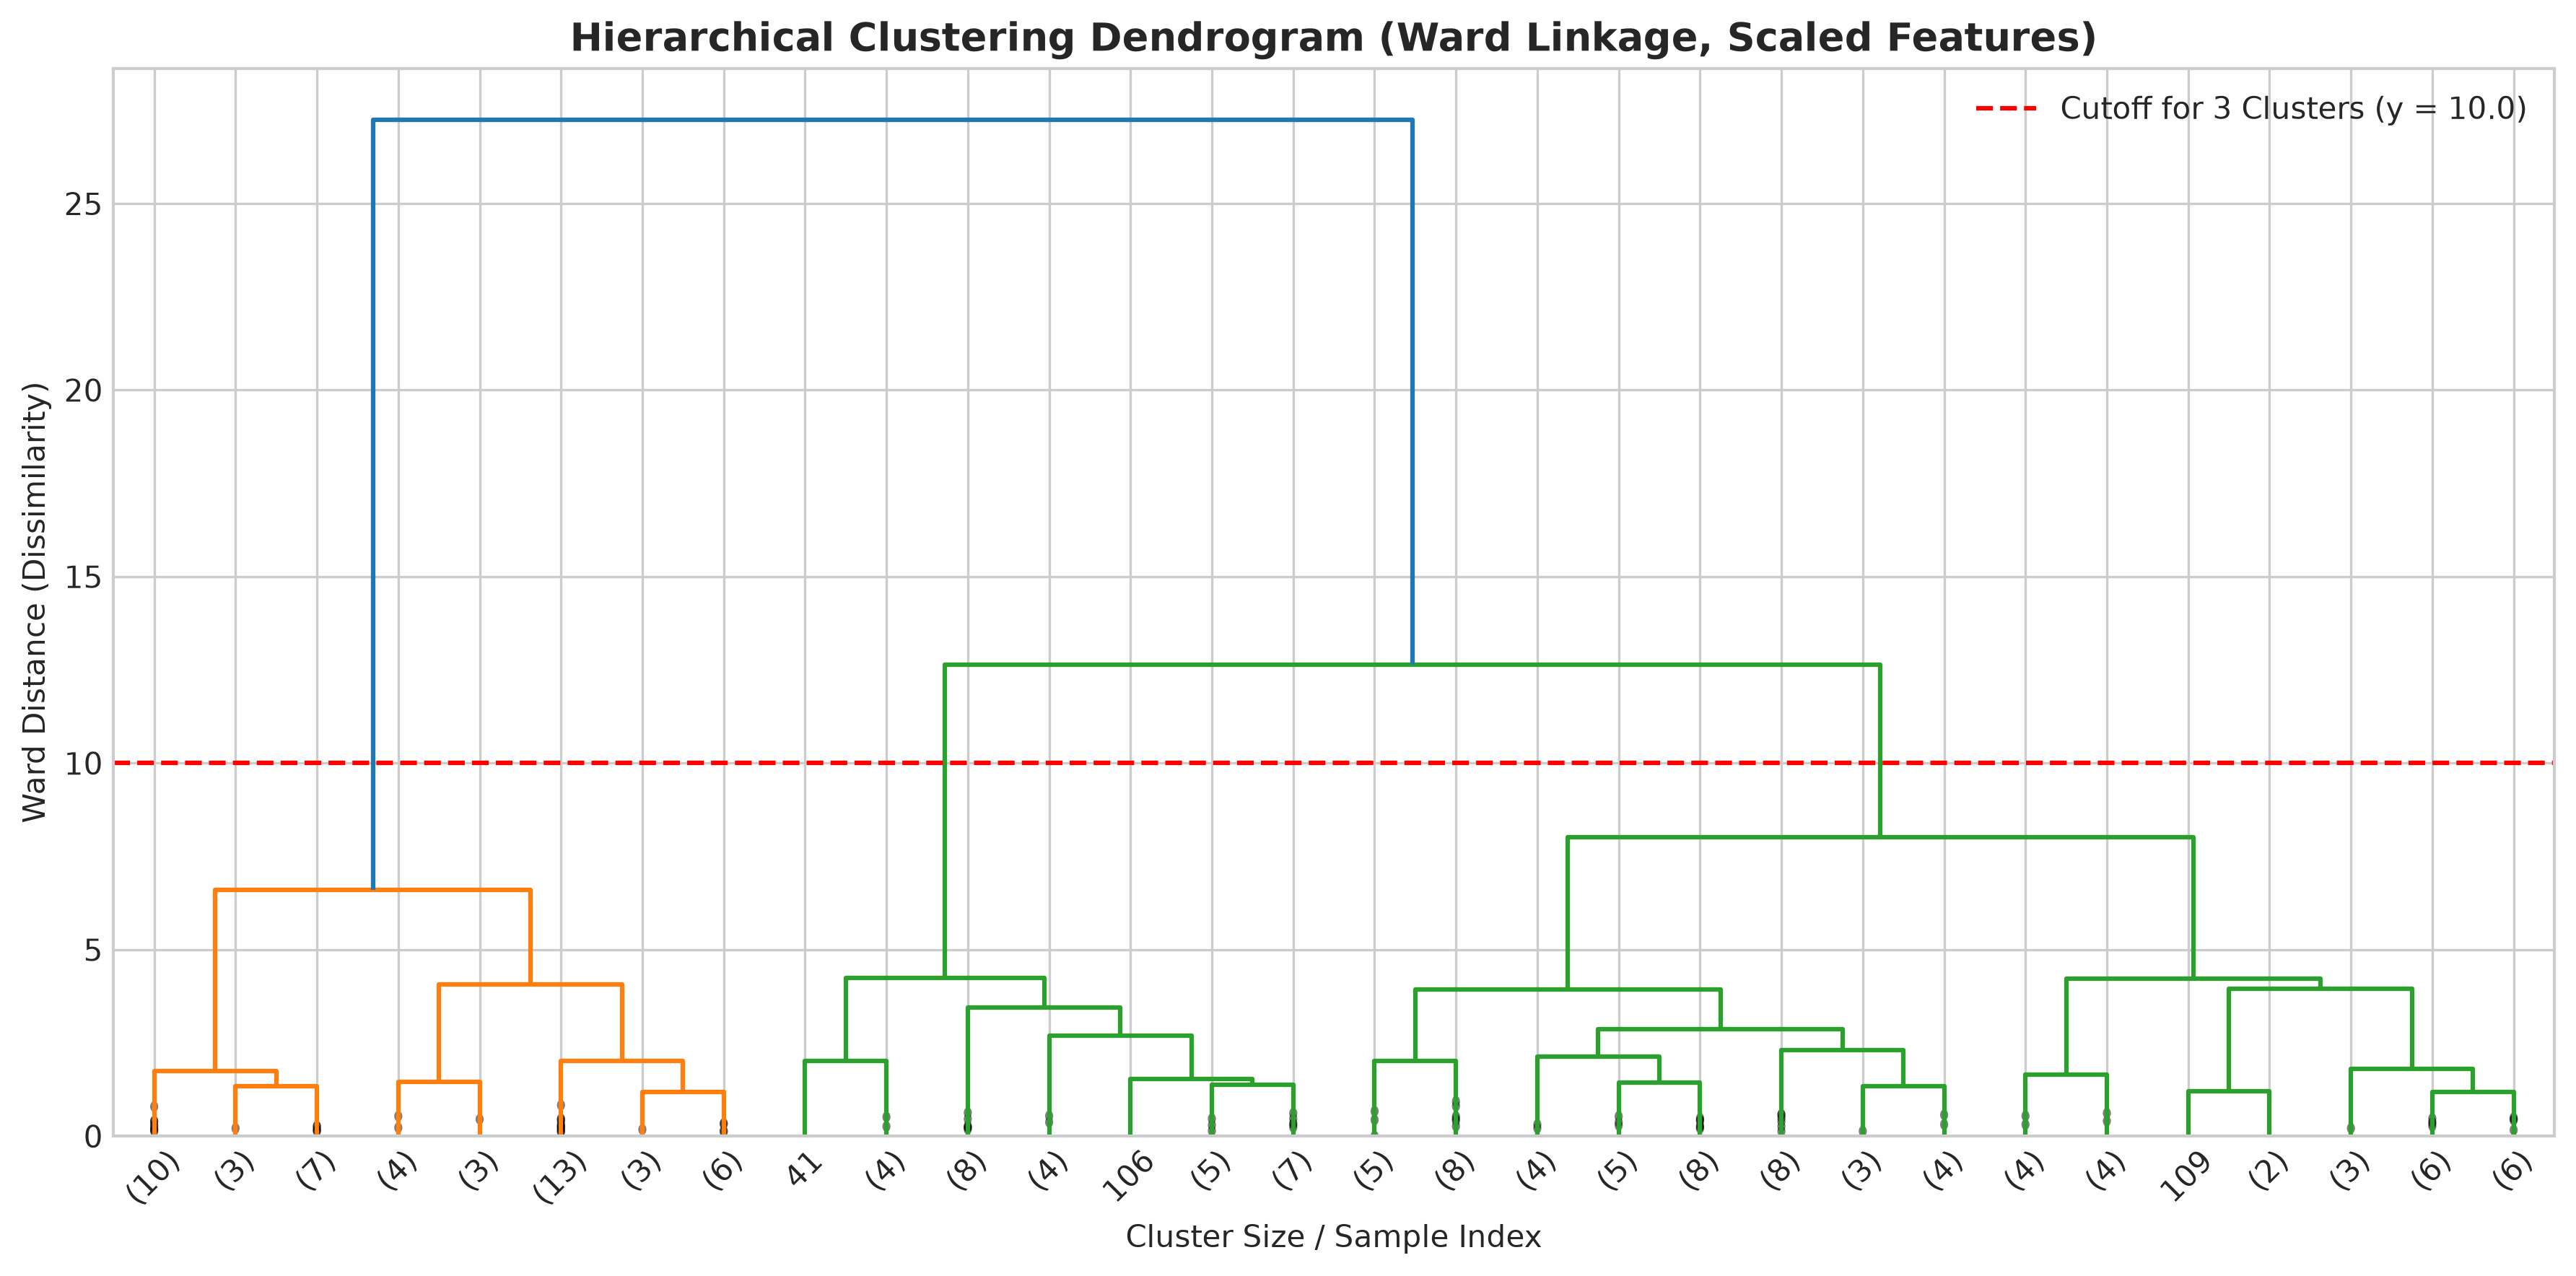
\includegraphics[width=0.92\linewidth]{figures/hierarchical_dendrogram.png}
    \caption{Hierarchical clustering dendrogram using Ward linkage on standardized features. The dashed red line at $y = 10.0$ establishes the threshold cut yielding 3 major clusters.}
    \label{fig:dendrogram}
\end{figure}

Cutting the dendrogram horizontally at dissimilarity threshold $y = 10.0$ yields three distinct subtrees, corroborating the structural suitability of $k=3$.

% =========================================================================
% SECTION 5: PERFORMANCE BENCHMARKING AND EVALUATION
% =========================================================================
\section{Performance Benchmarking and Quantitative Validation}

\subsection{Evaluation Metrics and Benchmark Comparison}
To validate clustering quality, both internal unsupervised geometric metrics and aligned external classification metrics against ground truth labels are computed.

\begin{lstlisting}[style=code, caption={Quantitative Performance Metric Computation}]
from sklearn.metrics import (
    silhouette_score, davies_bouldin_score, calinski_harabasz_score,
    confusion_matrix, mean_absolute_error, mean_squared_error
)

# Unsupervised and Supervised Benchmark Dictionary
metrics = {
    "Silhouette Score": [
        silhouette_score(X_scaled, kmeans_labels),
        silhouette_score(X_scaled, hier_labels)
    ],
    "Davies-Bouldin Index": [
        davies_bouldin_score(X_scaled, kmeans_labels),
        davies_bouldin_score(X_scaled, hier_labels)
    ],
    "Calinski-Harabasz Index": [
        calinski_harabasz_score(X_scaled, kmeans_labels),
        calinski_harabasz_score(X_scaled, hier_labels)
    ],
    "MAE": [mean_absolute_error(y, kmeans_aligned), mean_absolute_error(y, hier_aligned)],
    "MSE": [mean_squared_error(y, kmeans_aligned), mean_squared_error(y, hier_aligned)],
    "RMSE": [np.sqrt(mean_squared_error(y, kmeans_aligned)), np.sqrt(mean_squared_error(y, hier_aligned))]
}

results_df = pd.DataFrame(metrics, index=["K-Means", "Hierarchical"])
print(results_df.round(4))
\end{lstlisting}

\begin{table}[H]
\centering
\caption{Quantitative Performance Benchmark of Clustering Algorithms}
\label{tab:metrics}
\begin{tabular}{lcccccc}
\toprule
\textbf{Algorithm} & \textbf{Silhouette} $\uparrow$ & \textbf{Davies-Bouldin} $\downarrow$ & \textbf{Calinski-Harabasz} $\uparrow$ & \textbf{MAE} $\downarrow$ & \textbf{MSE} $\downarrow$ & \textbf{RMSE} $\downarrow$ \\
\midrule
\textbf{K-Means ($k=3$)} & \textbf{0.4599} & 0.8336 & \textbf{241.9044} & \textbf{0.1667} & \textbf{0.1667} & \textbf{0.4082} \\
\textbf{Hierarchical (Ward)} & 0.4467 & \textbf{0.8035} & 222.7192 & 0.1733 & 0.1733 & 0.4163 \\
\bottomrule
\end{tabular}
\end{table}

\begin{figure}[H]
    \centering
    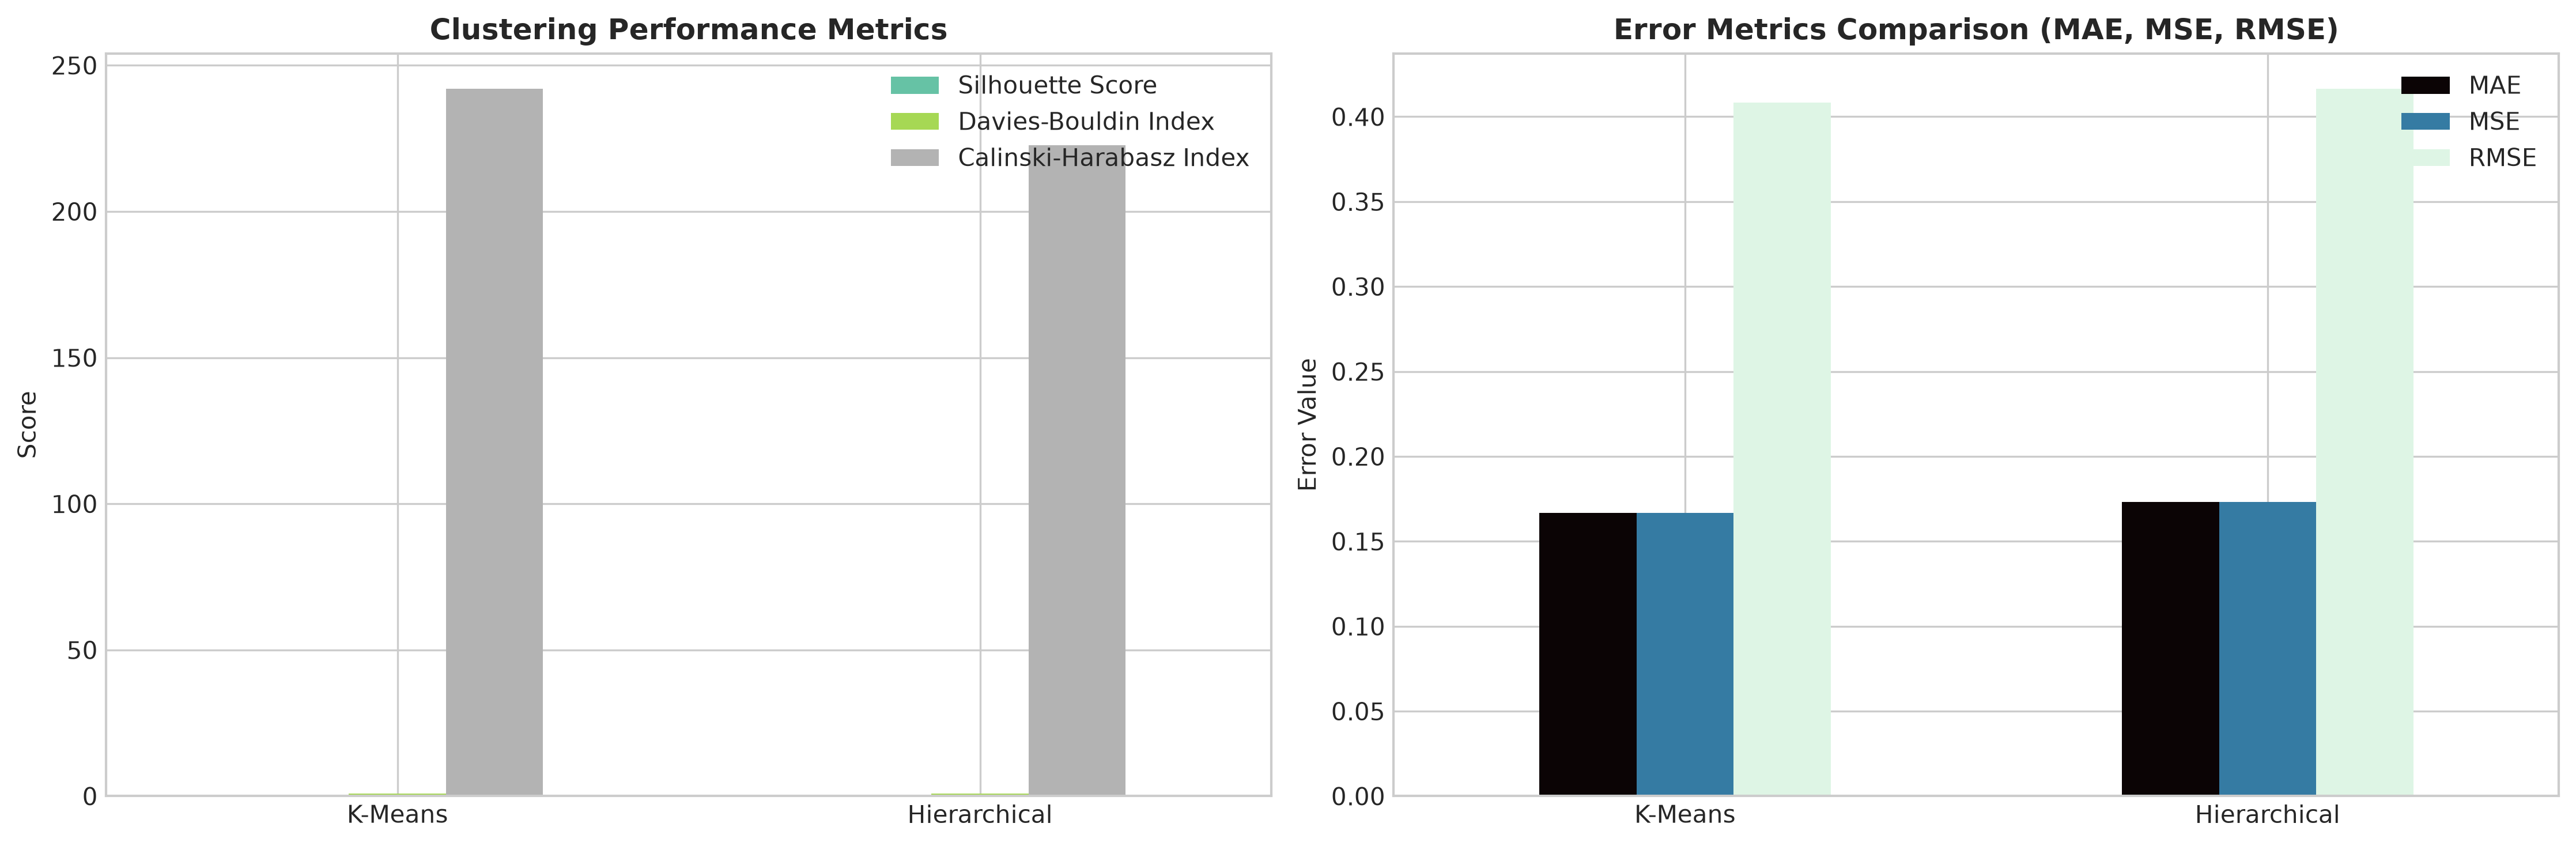
\includegraphics[width=0.95\linewidth]{figures/metrics_comparison_barcharts.png}
    \caption{Comparative performance metrics: (Left) Unsupervised validation indices (Silhouette, Davies-Bouldin, Calinski-Harabasz); (Right) Alignment error metrics (MAE, MSE, RMSE).}
    \label{fig:metrics_bar}
\end{figure}

\subsection{Cluster Alignment and Confusion Matrix Analysis}
Unsupervised cluster IDs are matched to ground-truth labels using majority voting alignment. The resulting confusion matrices are presented in Figure~\ref{fig:confusion_matrices}.

\begin{lstlisting}[style=code, caption={Majority Voting Cluster Alignment and Confusion Matrix Extraction}]
from scipy.stats import mode

def align_clusters(labels, true_labels):
    aligned = np.zeros_like(labels)
    for c in np.unique(labels):
        mask = (labels == c)
        true_mode = mode(true_labels[mask], keepdims=True).mode[0]
        aligned[mask] = true_mode
    return aligned

kmeans_aligned = align_clusters(kmeans_labels, y)
hier_aligned = align_clusters(hier_labels, y)

cm_kmeans = confusion_matrix(y, kmeans_aligned)
cm_hier = confusion_matrix(y, hier_aligned)
\end{lstlisting}

\begin{figure}[H]
    \centering
    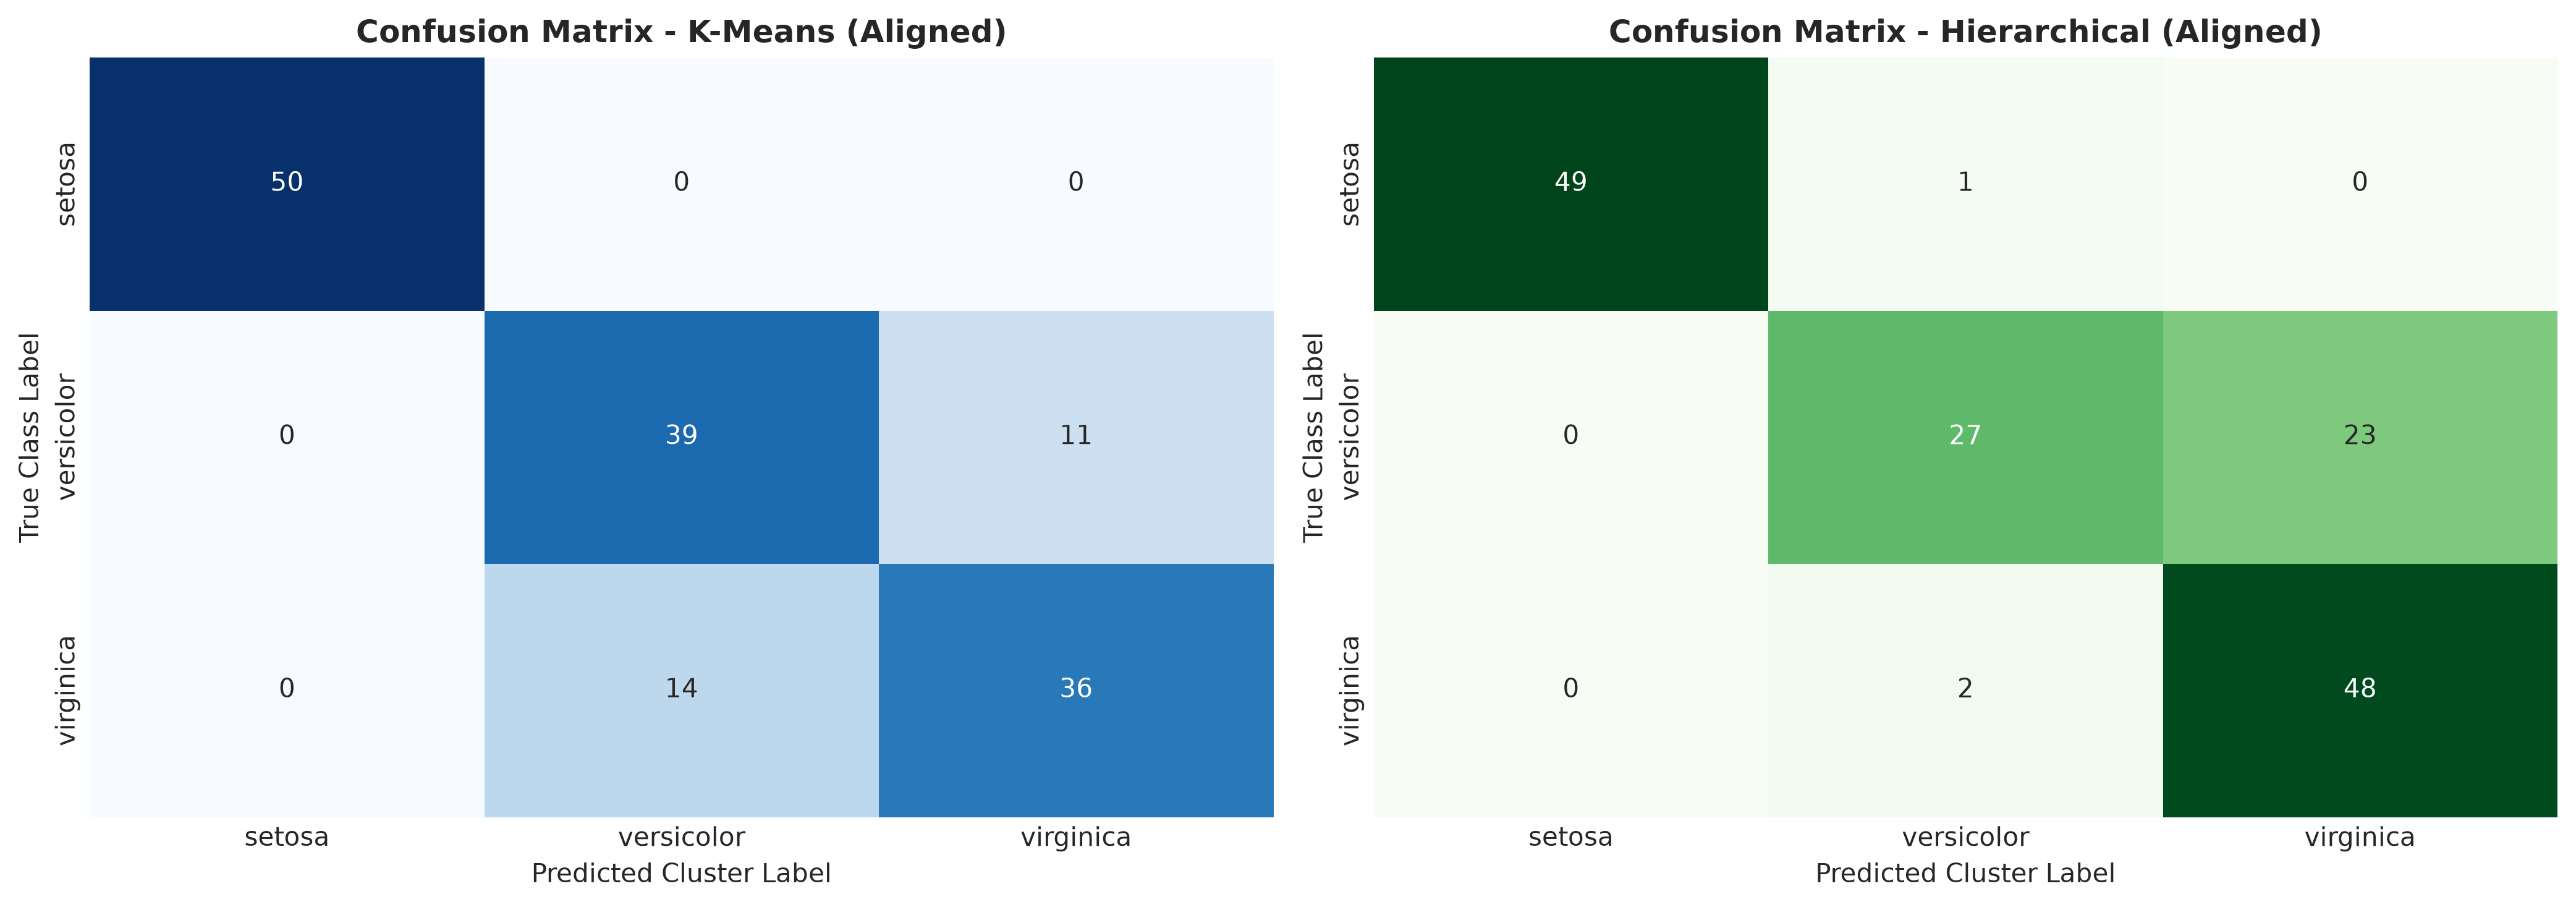
\includegraphics[width=0.92\linewidth]{figures/confusion_matrices.png}
    \caption{Confusion matrices for aligned K-Means (Left) and Hierarchical Clustering (Right) evaluated against ground-truth Iris species.}
    \label{fig:confusion_matrices}
\end{figure}

\textbf{Contingency Breakdown}:
\begin{itemize}
    \item \textbf{K-Means}: Accurately clusters all 50 \textit{Setosa} instances ($100\%$). For \textit{Versicolor}, 39 instances are classified correctly while 11 overlap into the \textit{Virginica} cluster. For \textit{Virginica}, 36 instances are classified correctly while 14 fall into the \textit{Versicolor} cluster. Total accuracy: $83.33\%$.
    \item \textbf{Hierarchical (Ward)}: Accurately clusters 49 \textit{Setosa} instances (1 placed in \textit{Versicolor}). For \textit{Versicolor}, 27 are grouped into cluster 1, while 23 bridge into the \textit{Virginica} cluster. For \textit{Virginica}, 48 are correctly grouped, with only 2 misassigned. Total accuracy: $82.67\%$.
\end{itemize}

% =========================================================================
% SECTION 6: DISCUSSION AND CONCLUSION
% =========================================================================
\section{Comparative Discussion and Conclusions}

\subsection{Comparative Algorithmic Tradeoffs}
\begin{table}[H]
\centering
\caption{Algorithmic Comparison: K-Means vs. Hierarchical Agglomerative Clustering}
\label{tab:comparison}
\begin{tabular}{p{3.5cm}p{5.5cm}p{5.5cm}}
\toprule
\textbf{Property} & \textbf{K-Means Clustering} & \textbf{Hierarchical (Ward)} \\
\midrule
\textbf{Computational Complexity} & $\mathcal{O}(N \cdot K \cdot d \cdot I)$ (Scalable to large datasets) & $\mathcal{O}(N^2 \log N)$ time, $\mathcal{O}(N^2)$ memory (Restricted to small/medium datasets) \\
\addlinespace
\textbf{Cluster Shape Assumption} & Convex, isotropic, spherical clusters around centroids & Flexible based on linkage (Ward favors equal-variance spherical clusters) \\
\addlinespace
\textbf{Determinism} & Stochastic (sensitive to centroid seed initialization) & Fully deterministic given distance matrix \\
\addlinespace
\textbf{Dendrogram Output} & No hierarchical hierarchy produced & Produces complete, cuttable multiscale tree \\
\addlinespace
\textbf{Best Performance Metric} & Higher Silhouette (0.4599) and Calinski-Harabasz (241.90) & Lower Davies-Bouldin Index (0.8035) \\
\bottomrule
\end{tabular}
\end{table}

\subsection{Analytical Insights}
\begin{enumerate}
    \item \textbf{Feature Scaling Necessity}: Preprocessing with $z$-score normalization is essential. Because Euclidean distance weights all dimensions equally, unscaled features with larger variance (such as Sepal Length) would dominate distance calculations and distort cluster topology.
    \item \textbf{Boundary Ambiguity}: Both algorithms cleanly separate \textit{Iris setosa} from the rest of the dataset due to substantial Euclidean margin in petal dimensions. However, the continuous morphometric gradient between \textit{Iris versicolor} and \textit{Iris virginica} leads to boundary crossover in both models, which aligns with biological taxonomy observations.
    \item \textbf{Metric Agreement}: K-Means achieves a slightly higher Silhouette score ($0.4599$ vs. $0.4467$) and Calinski-Harabasz score ($241.90$ vs. $222.72$), while Hierarchical clustering achieves superior Davies-Bouldin compactness ($0.8035$ vs. $0.8336$).
\end{enumerate}

\subsection{Conclusion}
This experimental study successfully implemented, evaluated, and compared K-Means and Hierarchical Agglomerative clustering on the Iris dataset. Hyperparameter sweeps using the Elbow Method and Silhouette analysis confirmed $k=3$ as the optimal natural partition count. Both algorithms achieved over $82\%$ unsupervised alignment with ground truth, demonstrating the power of geometric distance-based partitioning for unsupervised feature discovery.

\end{document}
